\documentclass{beamer}

\mode<presentation>
{
  \usetheme{CambridgeUS}
  \setbeamercovered{transparent}
  \setbeamertemplate{itemize items}[circle]
  \setbeamercolor{itemize item}{fg=red}%{\color{red}$\blacksquare$}
  \setbeamercolor{itemize subitem}{fg=gray}%{\color{gray}$\blacktriangleright$}
}

\usepackage[english]{babel}
\usepackage[latin1]{inputenc}
\usepackage{times}
\usepackage[T1]{fontenc} 
% Or whatever. Note that the encoding and the font should match. If T1
% does not look nice, try deleting the line with the fontenc.
\usepackage{amsmath}
\usepackage{hyperref}

\newcommand{\linespace}{\vskip 0.25cm}

%\definecolor{MyForestGreen}{rgb}{0,0.7,0} 
%\newcommand{\tableemph}[1]{{#1}}
%\newcommand{\tablewin}[1]{\tableemph{#1}}
%\newcommand{\tablemid}[1]{\tableemph{#1}}
%\newcommand{\tablelose}[1]{\tableemph{#1}}

%\definecolor{MyLightGray}{rgb}{0.6,0.6,0.6}
%\newcommand{\tabletie}[1]{\color{MyLightGray} {#1}}

% The text in square brackets is the short version of your title and will be used in the
% header/footer depending on your theme.
\title[Foveated Rendering]{Foveated rendering \\ in virtual reality}

% Sub-titles are optional - uncomment and edit the next line if you want one.
% \subtitle{Why does sub-tree crossover work?} 

% The text in square brackets is the short version of your name(s) and will be used in the
% header/footer depending on your theme.
\author[Miller]{Sam Miller}

% The text in square brackets is the short version of your institution and will be used in the
% header/footer depending on your theme.
\institute[U of Minn, Morris]
{
  Division of Science and Mathematics \\
  University of Minnesota, Morris \\
  Morris, Minnesota, USA
}

% The text in square brackets is the short version of the date if you need that.
\date[October '17] % (optional)
{October 2017}

% Delete this, if you do not want the table of contents to pop up at
% the beginning of each subsection:
%\AtBeginSection[]
%{
%  \begin{frame}<beamer>
%    \frametitle{Outline}
%    \tableofcontents[currentsection, hideothersubsections]
%  \end{frame}
%}

\begin{document}

\begin{frame}
  \titlepage
\end{frame}

% For a 20-25 minute senior seminar talk you probably want something like:
% - Two or three major sections (other than the summary).
% - At *most* three subsections per section.
% - Talk about 30s to 2min per frame. So there should probably be between
%   15 and 30 frames, all told.

\section*{Overview}

\subsection*{Outline}

\begin{frame}
  \frametitle{Outline}
  	%\tableofcontents[hideallsubsections]
  	
	\begin{itemize}
    \item Background
	\begin{itemize}
    \item Human Vision
    \item Gaze Tracking
    \item Virtual Reality Headsets
    \linespace
	\end{itemize}
	\item Foveated Renderer Design
	\begin{itemize}
    \item Desktop Implementation
    \item VR Implementation
    \linespace
	\end{itemize}
	\item Results
	\linespace
	\item Conclusion
	\end{itemize}
	

\end{frame}

\section[Introduction]{Background}

\subsection{Background}

\begin{frame}
  \frametitle{Utilizing foveated rendering}
  
  %\begin{columns}
  %\begin{column}{.65\textwidth}
Foveated rendering is a valuable tool for reducing computational load when rendering three-dimensional scenes.

\linespace

There are several critical factors that must be handled when implementing one of these renderers.

%\linespace

  %\end{column}
  \begin{center}
    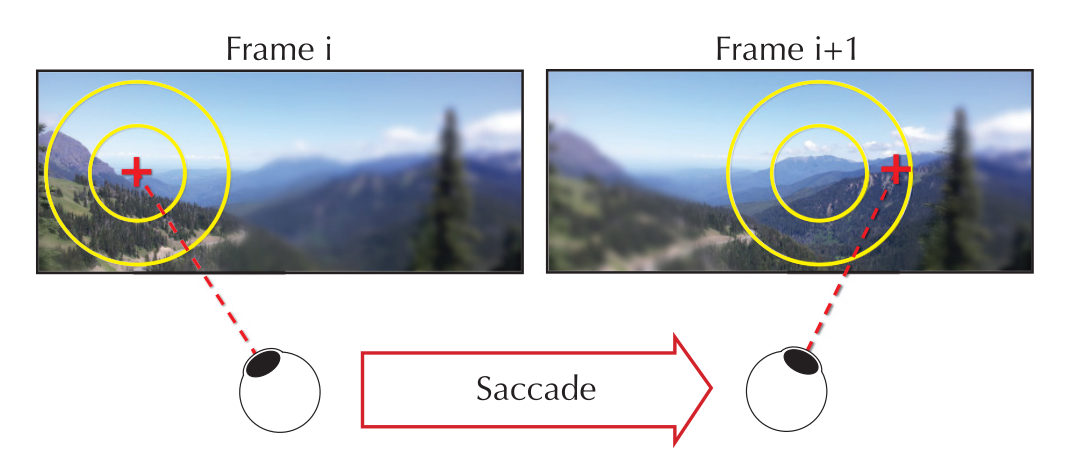
\includegraphics[width=.95\textwidth]{Illustrations/saccade.png}
    \\
    %\tiny{Sam Fraser-Smith \\ \url{http://tr.im/pq7l} }
  \end{center}
  
\end{frame}

\begin{frame}
\frametitle{Hardware advancement}

\begin{columns}
\begin{column}{0.5\textwidth}

\begin{itemize}
	\item Early implementations of this technique used hardware such as the NAC Eye Mark eye Tracker (pictured top right).
	\linespace
	\item Current implementations (as of 2017) can use the existing setup of high profile VR HMDs.
	\linespace
	\item This technology is becoming more in demand as the VR userbase expands.
\end{itemize}
\end{column}

\begin{column}{0.02\textwidth}
\end{column}

\begin{column}{0.5\textwidth}

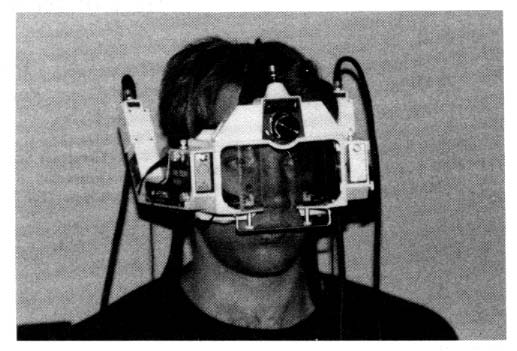
\includegraphics[width=0.715\textwidth]{Illustrations/gazeTracker.png}

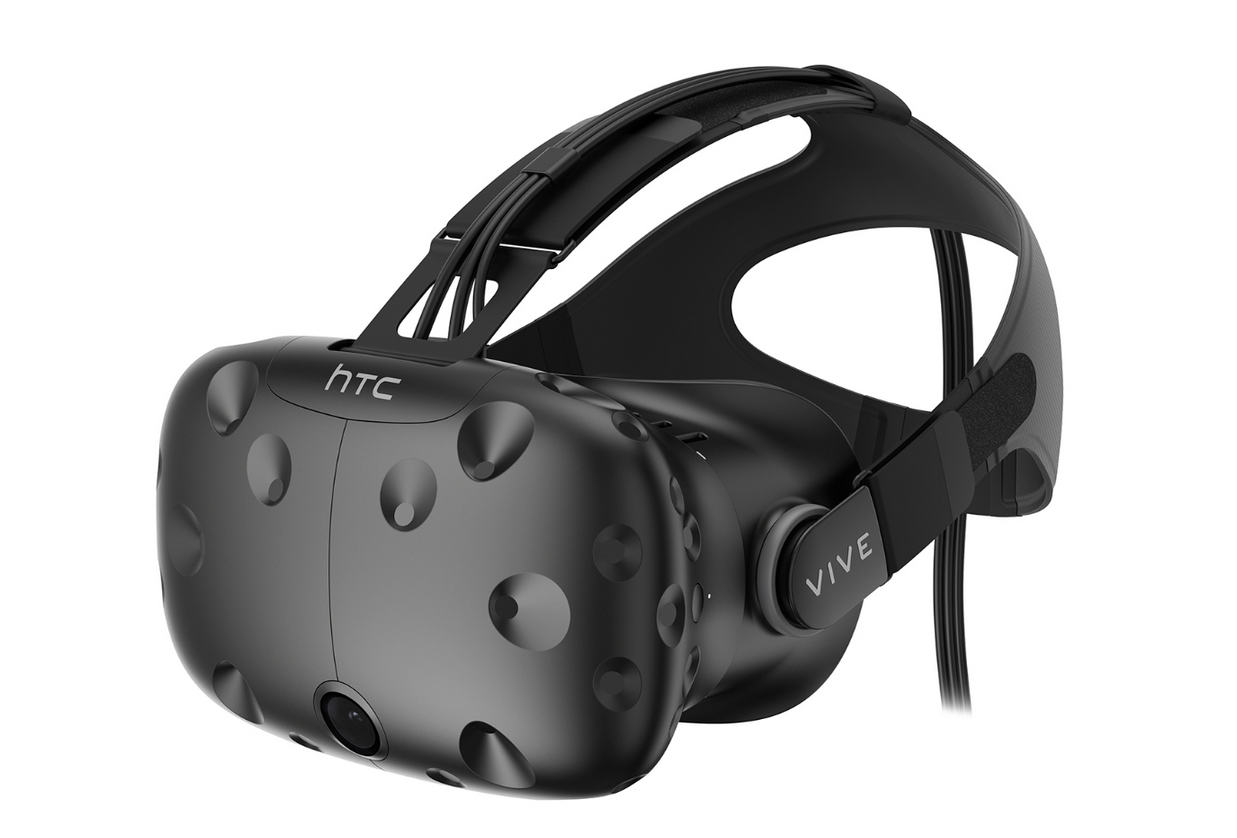
\includegraphics[width=0.715\textwidth]{Illustrations/vive.png}

\end{column}
\end{columns}

\end{frame}

\section[Conclusion]{Questions}

\begin{frame}
	\frametitle{Thanks}

	\begin{center}
	{\huge Questions?}
	\end{center}
\end{frame}


\end{document}


